\section{\esp Introdução}

O problema dos k-centros é um desafio de otimização utilizado em técnicas de \textit{clustering}, onde o objetivo é encontrar \textbf{k} centros no espaço de dados que minimizem a maior distância entre um ponto e seu centro mais próximo. Esse problema é frequentemente utilizado em problemas de alocação de recursos, roteamento de veículos e análise de agrupamentos.

Dado um grafo com vértices representando os pontos de dados, o objetivo é selecionar \textit{k} vértices como centros de \textit{clusters}, de forma que a soma das distâncias entre cada ponto de dados e seu centro mais próximo seja minimizada. Essa distância pode ser medida de diferentes maneiras, como a distância euclidiana ou a distância de Manhattan.

Dentre as possíveis soluções para o problema exploramos aqui duas delas: o algoritmo de \textbf{Força Bruta} e o algoritmo de \textbf{\textit{Minimum Spanning Tree} (MST)}. O método de \textbf{Força Bruta} verifica todas as possíveis combinações de centros e seleciona a alocação que minimiza a maior distância. No entanto, esse método é computacionalmente caro e inviável para grandes conjuntos de dados. Quanto ao \textbf{MST}, a ideia básica do algoritmo é encontrar uma árvore geradora mínima do grafo usando um algoritmo eficiente, como o algoritmo de Kruskal ou o algoritmo de Prim. Uma vez que ela é construída, cada centro é escolhido como o vértice com maior distância em relação aos centros já selecionados. Esse algoritmo é baseados em heurísticas que buscam encontrar uma solução aproximada, mas geralmente eficiente, para o problema. 

Neste trabalho, exploramos possíveis soluções para o problema apresentado utilizando as instâncias disponíveis pela OR-Library. Ao fim do trabalho, foram comparados os resultados adquiridos com os resultados esperados, no intuito de avaliar o desempenho dos algoritmos implementados. 

\section{\esp IMPLEMENTAÇÃO}

Para desenvolver a solução do trabalho, utilizamos a linguagem Python. Ela foi escolhida por ser uma linguagem rápida e eficiente. 

Em uma mesma \textit{Thread} de execução, foram implementadas as classes \textit{bruce\_force\_solver} e \textit{mst\_solver} para solucionar o problema dos k-centros dos grafos. Além disso, várias outras classes complementares também foram implementadas para que, agrupadamente, formassem a solução do problema.  


\subsection{\esp Classe Grafo}
A classe \textbf{Grafo} possui os atributos \textit{\_is\_directional}, \textit{\_num\_edges}, \textit{\_num\_nodes}, \textit{\_k\_centers} e \textit{\_edges\_weights} que representam, respectivamente, se o grafo é direcionado, o número de arestas, o número de vértices, o número de k-centros e os pesos das arestas. Além disso, a classe é composta por diversos métodos, dentre eles, os principais são: \textit{from\_file}, que cria e retorna os grafos a partir dos arquivos de entrada, \textit{get\_min\_distance} que utiliza o algoritmo de Floyd-Warshall para calcular as distâncias mínimas, \textit{set\_edge} que atribui os pesos das arestas sendo que, se a aresta não existir, ele atribui o peso a ela, e se ela já existir, ele atribui o menor peso a ela, \textit{calculate\_excentricity}, que calcula e retorna a excentricidade de um nó do grafo utilizando o algoritmo de busca de custo uniforma, que garante encontrar uma solução se ela existir, \textit{get\_reachable\_nodes}, que retorna uma lista de nós alcançáveis a partir de um determinado nó usando busca em largura, e, por fim, \textit{is\_reachable\_from}, que verifica se um nó específico é alcançável a partir de outro nó do grafo utilizando o método de busca em largura para executar a pesquisa.

Foi utilizada a estrutura de matriz de adjacência para armazenar as arestas dos grafos e seus respectivos pesos. Essa estrutura foi escolhida por permitir acessar rapidamente o peso de uma aresta entre dois vértices, bastando apenas acessar o valor correspondente na matriz. 


\subsection{\esp Algoritmos}

Para solucionar o problema apresentado neste documento, a primeira abordagem tomada é a \textbf{Força Bruta}, que garante encontrar a melhor solução ao custo da performance do algoritmo. Este método considera todas as combinações possíveis de centros e calcula o raio máximo para cada combinação, apresentando uma solução precisa e ótima. 

A segunda abordagem tomada é o algoritmo de \textbf{Árvore Geradora Mínima (MST)}, que encontra soluções aproximadas para o problema, mas apresenta melhor eficiência em termos de tempo de execução, principalmente para grafos grandes. Ele constrói uma árvore geradore mínima no grafo e encontra os centros com base na excentricidade dos nós. 

\subsubsection{\esp Algoritmo de Força Bruta}
O algoritmo utiliza força bruta para testar todas as combinações possíveis de centros e calcular o raio mínimo de alcance deles, garantindo a solução ótima para o problema de se encontrar os melhores centros do grafo. 

O construtor da classe \textit{BruteForceSolver} recebe como entrada um objeto Grafo e o número \textit{k\_centros} que indica a quantidade de centros a serem encontrados. O método \textit{find\_best\_centers} é o ponto de entrada do algoritmo e retorna os melhores centros encontrados e o raio mínimo de alcance. Ele inicializa variáveis como \textit{centers}, \textit{best\_centers} e \textit{min\_radius} para acompanhar os melhores centros encontrados até o momento. O algoritmo usa um loop para testar cada quantidade de centros, de 1 até \textit{k\_centros}. 

Dentro do loop, o método \textit{find\_best\_center\_ite} é chamado para encontrar os melhores centros para a quantidade atual de centros. Ele utiliza, então, outro loop para gerar todas as combinações possíveis de nós para os centros, utilizando o algoritmo clássico de geração de combinações. Para cada combinação de centros, o algoritmo distribui os nós restantes para os centros mais próximos, calculando as distâncias e armazenando em uma estrutura de dados. Em seguida, ele encontra o raio máximo de alcance para a distribuição atual e atualiza as variáveis \textit{best\_centers} e \textit{min\_radius} se o raio atual for menor do que o mínimo encontrado até o momento. O loop continua gerando todas as combinações possíveis até que todas sejam testadas. Ao final, o algoritmo retorna os melhores centros encontrados  e o raio mínimo de alcance.

Apesar de garantir a solução ótima, essa abordagem pode ser computacionalmente intensiva para grafos grandes, já que o número de combinaçõs cresce exponencialmente com o número de nós. Por este motivo, foi implementado, também, um limite de tempo para evitar execuções muito longas. 


\subsubsection{\esp Algoritmo de Árvores Geradoras}
O algoritmo é um solver baseado na construção de uma floresta de árvores de espalhamento mínimo \textit{(MSF - Minimum Spanning Forest)} com prioridade uma fila para encontrar os melhores centros em um grafo.  Foi utilizado o método \textit{get\_run\_time} para calcular o tempo de execução.

A classe \textit{MSTSolver} recebe o grafo e o número de centros desejados como entrada. O método \textit{build\_ms\_forest\_} constrói a \textit{Minimum Spanning Tree (MST)} do grafo utilizando uma fila de prioridade para otimizar o processo. As arestas são adicionadas à fila juntamente com o seu peso. Enquanto houver arestas na fila de prioridade e o número de arestas na MSF for menor que o número de nós - número de centros, o algoritmo continua iterando. A cada iteração, uma aresta é removida da fila de prioridade e é verificado se ela conecta dois nós que ainda não são alcançáveis na MSF. Se sim, a aresta é adicionada à MSF e é feita uma verificação adicional para manter a propriedade da MSF. Essa propriedade é mantida verificando se a excentricidade do menor caminho entre os nós alcançáveis na MSF é maior que o peso mínimo na fila de prioridade. Se for, a aresta é removida da MSF e adicionada novamente à fila de prioridade com um novo peso igual à excentricidade. Durante o processo, também são realizadas verificações para evitar a formação de ciclos no grafo.

O método \textit{find\_best\_centers} recebe uma matriz \textit{subgraphs} que representa as subárvores geradoras encontradas. O método percorre cada subgrafo e calcula a excentricidade de cada vértice em relação aos outros vértices do mesmo subgrafo. Em seguida, seleciona o vértice com a menor excentricidade como centro do subgrafo e retorna uma lista contendo os melhores centros encontrados e o raio mínimo alcançado.

O método \textit{calculate\_component\_radius} calcula o raio de um componente em um grafo representado por uma matriz. Ele recebe uma matriz e um vértice como entrada e retorna o raio do componente.

Este algoritmo geralmente é mais eficiente do que a abordagem de força bruta quando o número de nós no grafo é grande. No entanto, a eficiência ainda pode depender do tamanho do grafo e da implementação específica.

\section{\esp Análise de resultados}
Nessa seção analisamos o desempenho dos algoritmos implementados analisando o tempo de execução e a precisão dos resultados obtidos por cada um. 

\subsection{\esp Experimentos}
Os algoritmos descritos na seção 2.2 foram executados em um processador Intel Core i5 de 8ª geração 1.80 GHz. Foram testadas diversas instâncias com diferentes tamanhos, o que afeta diretamente o desepenho apresentado pelos algoritmos. Por este motivo, foi implementado um limite de tempo de 1 hora de execução para cada instância. Quando este limite é alcançado, a execução é abortada e o melhor resultado encontrado até então é retornado. 

\subsection{\esp Resultados}
Os resultados dos valores de k-centros e seus respectivos raios encontrados para cada instância são apresentados na Tabela 1. A Figura 1 representa esses resultados em um gráfico. Para todas as instâncias, o algoritmo MST encontrou os valores de k-centros corretos, mas de raios diferentes da solução. Os raios encontrados representam a solução aproximada implementada pelo algoritmo. 

\begin{figure}[h]
  \centering
  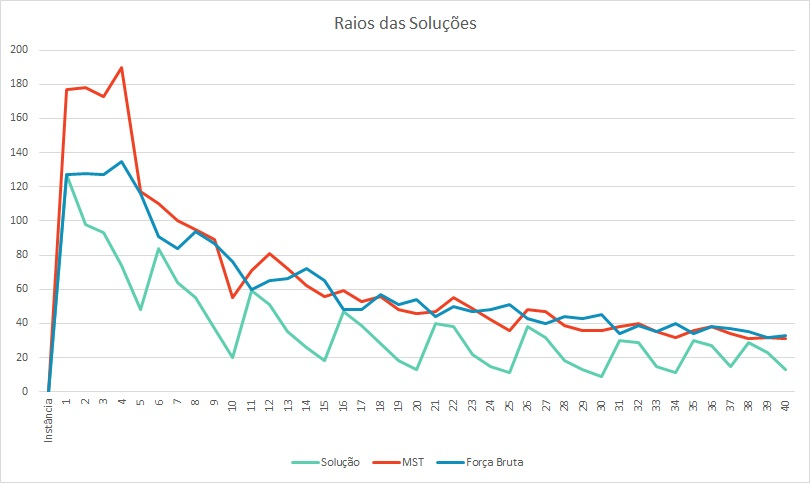
\includegraphics[width=1.0\textwidth]{figuras/raios.jpg}
  \caption{Raios obtidos pelos algoritmos MST e Força Bruta}
  \label{fig:raios}
\end{figure}

Já o algoritmo de Força Bruta, que devido ao tempo limite de uma hora implementado, só conseguiu realizar a busca completa da primeira instância, e encontrou a solução ótima para esta. Para as demais instâncias, o algoritmo realizou a busca durante o tempo limite e apresentou os resultados obtidos até então. Estes raios obtidos, são, portanto, uma solução aproximada também. Entretanto, vale ressaltar que, com o uso de computadores mais potentes ou maior tempo limite, a solução ótima poderia ser encontrada para todas as instâncias utilizando este algoritmo. 


\begin{table}[h]
	\centering
	\caption{\hspace{0.1cm} Resultados obtidos para os algoritmos}
	\vspace{-0.3cm} % espaço entre titulo e tabela
	\label{tab:tabela1}
	% Conteúdo da tabela
	\begin{tabular}{c|c|c|c|c|c|c|c}
		\hline
		 \multicolumn{2}{c|}{ }& \multicolumn{2}{c|}{Solução} & \multicolumn{2}{c|}{MST} & \multicolumn{2}{c|}{Força bruta}\\ 
		\hline
		\textbf{Instância} & $\vert V \vert$ & $k$ & Raio & $k$ & Raio & $k$ & Raio  \\
		\hline
		1 & 100 & 5 & 127 & 5 & 177 & 5 & 127 \\
		2 & 100 & 10 & 98 & 10 & 178 & 5 (TIMEOUT) & 128 (TIMEOUT)\\
		3 & 100 & 10 & 93 & 10 & 173 & 5 (TIMEOUT) & 127 (TIMEOUT)\\
		4 & 100 & 20 & 74 & 20 & 190 & 5 (TIMEOUT) & 135 (TIMEOUT)\\
		5 & 100 & 33 & 48 & 33 & 117 & 5 (TIMEOUT) & 116 (TIMEOUT)\\
		6 & 200 & 5 & 84 & 5 & 110 & 4 (TIMEOUT) & 91 (TIMEOUT)\\
		7 & 200 & 10 & 64 & 10 & 100 & 5 (TIMEOUT) & 84 (TIMEOUT)\\
		8 & 200 & 20 & 55 & 20 & 95 & 4 (TIMEOUT) & 94 (TIMEOUT)\\
		9 & 200 & 40 & 37 & 40 & 89 & 4 (TIMEOUT) & 87 (TIMEOUT)\\
		10 & 200 & 67 & 20 & 67 & 55 & 4 (TIMEOUT) & 76 (TIMEOUT) \\
		11 & 300 & 5 & 59 & 5 & 71 & 4 (TIMEOUT) & 60 (TIMEOUT)\\
		12 & 300 & 10 & 51 & 10 & 81 & 4 (TIMEOUT) & 65 (TIMEOUT)\\
		13 & 300 & 30 & 35 & 30 & 72 & 4 (TIMEOUT) & 66 (TIMEOUT)\\
		14 & 300 & 60 & 26 & 60 & 62 & 4 (TIMEOUT) & 72 (TIMEOUT)\\
		15 & 300 & 100 & 18 & 100 & 56 & 3 (TIMEOUT) & 65 (TIMEOUT)\\
		16 & 400 & 5 & 47 & 5 & 59 & 3 (TIMEOUT) & 48 (TIMEOUT)\\
		17 & 400 & 10 & 39 & 10 & 53 & 4 (TIMEOUT) & 48 (TIMEOUT)\\
		18 & 400 & 40 & 28 & 40 & 56 & 3 (TIMEOUT) & 57 (TIMEOUT)\\
		19 & 400 & 80 & 18 & 80 & 48 & 3 (TIMEOUT) & 51 (TIMEOUT)\\
		20 & 400 & 133 & 13 & 133 & 46 & 4 (TIMEOUT) & 54 (TIMEOUT)\\
		21 & 500 & 5 & 40 & 5 & 47 & 3 (TIMEOUT) & 44 (TIMEOUT) \\
		22 & 500 & 10 & 38 & 10 & 55  & 3 (TIMEOUT) & 50 (TIMEOUT)\\
		23 & 500 & 50 & 22 & 50 & 49  & 3 (TIMEOUT) & 47 (TIMEOUT)\\
		24 & 500 & 100 & 15 & 100 & 42 & 3 (TIMEOUT) & 48 (TIMEOUT) \\
		25 & 500 & 167 & 11 & 167 & 36 & 3 (TIMEOUT) & 51 (TIMEOUT) \\
		26 & 600 & 5 & 38 & 5 & 48 & 3 (TIMEOUT) & 43 (TIMEOUT) \\
		27 & 600 & 10 & 32 & 10 & 47  & 3 (TIMEOUT) & 40 (TIMEOUT)\\
		28 & 600 & 60 & 18 & 60 & 39 & 3 (TIMEOUT) & 44 (TIMEOUT) \\
		29 & 600 & 120 & 13 & 120 & 36  & 3 (TIMEOUT) & 43 (TIMEOUT)\\
		30 & 600 & 200 & 9 & 200 & 36 & 3 (TIMEOUT) & 45 (TIMEOUT) \\
		31 & 700 & 5 & 30 & 5 & 38  & 3 (TIMEOUT) & 34 (TIMEOUT)\\
		32 & 700 & 10 & 29 & 10 & 40  & 3 (TIMEOUT) & 39 (TIMEOUT)\\
		33 & 700 & 70 & 15 & 70 & 35 & 3 (TIMEOUT) & 35 (TIMEOUT)\\
		34 & 700 & 140 & 11 & 140 & 32 & 3 (TIMEOUT) & 40 (TIMEOUT)\\
		35 & 800 & 5 & 30 & 5 & 36 & 3 (TIMEOUT) & 34 (TIMEOUT)\\
		36 & 800 & 10 & 27 & 10 & 38 & 3 (TIMEOUT) & 38 (TIMEOUT) \\
		37 & 800 & 80 & 15 & 80 & 34 & 3 (TIMEOUT) & 37 (TIMEOUT) \\
		38 & 900 & 5 & 29 & 5 & 31 & 3 (TIMEOUT) & 35 (TIMEOUT)\\
		39 & 900 & 10 & 23 & 10 & 32 & 3 (TIMEOUT) & 32 (TIMEOUT)\\
		40 & 900 & 90 & 13 & 90 & 31 & 3 (TIMEOUT) & 33 (TIMEOUT)\\
		\hline
	\end{tabular}
	\vspace{.1cm} %espaço entre tabela e fonte
	\small
	% Fonte
	{\footnotesize\\ \textbf{Fonte:} Dados da pesquisa}
\end{table}


\subsection{\esp Análise Comparativa}
Ao implementar o algoritmo MST para encontrar os k-centros dos grafos, todas as instâncias foram processadas sem exceder o tempo limite de uma hora previamente estipulado. Entretanto, os valores obtidos para os raios das soluções são valores aproximados, já que essa abordagem encontra os k-centros do grafo em relação à àrvore geradora mínima do mesmo, não levando em consideração todas as possíveis combinações dos vértices. Esse método se apresentou mais eficiente do que a abordagem de força bruta quando o número de nós no grafo é grande. No entanto, ele não é capaz de fornecer uma solução ótima para o problema.

Para o algoritmo de Força Bruta, os resultados obtidos mostram que para todas as instâncias exceto a 1, o limite de tempo de 1 hora previamente estipulado foi atingido. Sendo assim, para estas instâncias, o resultado obtido foi aproximado. Isso ocorre devido à quantidade de combinações que o algoritmo realiza para se obter o resultado.  A complexidade de tempo é alta, sendo exponencial em relação ao número de centros (k\_centros) e ao número de nós no grafo. Como essa abordagem envolve a enumeração de todas as possíveis combinações de k-vértices, além do cálculo da soma das distâncias entre cada vértice a seu centro mais próximo, sua eficiência diminui rapidamente à medida que o tamanho do problema aumenta.


\section{\esp Conclusão}
A matriz de adjacência permite acessar rapidamente o peso de uma aresta entre dois nós, pois basta acessar o valor correspondente na matriz. No entanto, essa representação consome mais espaço em memória em comparação com outras estruturas de dados, especialmente para grafos densos (com muitas arestas). Além disso, o custo para percorrer todos os vizinhos de um nó é proporcional ao número total de nós no grafo, o que pode ser ineficiente para grafos com muitos nós.

Em termos de eficiência, o algoritmo de MST foi capaz de processar todas as instâncias em tempo hábil, se mostrando eficiente. Já o algortimo de força bruta, devido à complexidade exponencial em relação ao número de vértices do grafo, se apresentou ineficiente à medida que o tamanhodo grafo aumenta.  

Quanto ao desempenho, o algoritmo MST, embora ainda tenha uma complexidade de tempo razoável, oferece uma solução aproximada com bom desempenho na maioria dos casos. Já o algoritmo de Força Bruta pode se tornar impraticável para grafos com grande número de vértices.

Por fim, avaliando agora a precisão dos métodos, o algoritmo de MST fornece uma solução aproximada, pois os centros são escolhidos com base nas excentricidades dos nós na MST. Já o algoritmo de Força Bruta considera todas as combinações possíveis, garantindo uma solução precisa e ótima. 

Conclui-se, então, que para grafos com números limitados de nós, o algoritmo de Força Bruta, apesar de apresentar tempo de execução elevado, é capaz de fornecer uma solução ótima. Entretanto, essa solução pode ser inviável para grafos maiores, sendo, então, a melhor opção, o algoritmo de MST, que garantirá uma solução aproximada em tempo hábil. 





